%Basic Formatting and Packages---------------------------------------------------------------------------------------------------------------------------------------------------------------------------
\documentclass[11pt,a4paper]{article}
\usepackage{amsmath} 
\usepackage{amssymb}   
\usepackage{graphicx}
\usepackage{geometry}
\usepackage{mathtools}
\usepackage[dvipsnames]{xcolor}
\usepackage{enumitem}
\usepackage{tcolorbox}
\usepackage{verbatim}
\usepackage{csvsimple}
\usepackage{subcaption}
\usepackage[font=tiny,labelfont=bf]{caption}
\usepackage{float}
\usepackage{listings}
\usepackage{hyperref}

\usepackage{longtable}
\usepackage{multirow}
\usepackage{array}
\usepackage{booktabs}
%\usepackage[ruled, noend]{algorithm2e}

\usepackage{tikz}
\usetikzlibrary{shapes.geometric, arrows, positioning}

\geometry{left=2cm,right=2cm,top=2.5cm,bottom=2.5cm}


\lstset{basicstyle=\footnotesize}



\title{\textbf{The influence of distribution characteristics and data balancing on classification bias in highly unbalanced data sets}}
    \author{
        \parbox{\linewidth}{\centering
            Zekiye Erarslan, Manuel Günther, Artemii Redkin, Matteo Zannini
        }
     }
    \date{30.09.2023}

\usepackage{newunicodechar}
\newunicodechar{⁠}{\nolinebreak}




\definecolor{myblue}{cmyk}{1,.72,0,.38}

% Define custom colors
%\definecolor{myblue}{rgb}{0,0,1}
\definecolor{myyellow}{rgb}{1,1,0}
\definecolor{myorange}{rgb}{1,0.5,0}
\definecolor{mypurple}{rgb}{0.5,0,0.5}
\definecolor{mygreen}{rgb}{0,0.5,0}

%Python code style settings---------------------------------------------------------------------------------------------------------------------------------------------------------------------------------------

% Define a custom style for Python code
\lstdefinestyle{mystyle}{
    backgroundcolor=\color{white},       % background color
    commentstyle=\color{mygreen},        % comment color
    keywordstyle=\color{mypurple},         % keyword color
    numberstyle=\tiny\color{gray},     % line numbers color
    stringstyle=\color{orange},       % string color 
    identifierstyle =\color{myblue},
    basicstyle=\ttfamily\scriptsize,          % code font and size
    breakatwhitespace=false,             % break lines only at whitespace
    breaklines=true,                     % enable line breaking
    captionpos=b,                        % caption position (bottom)
    keepspaces=true,                     % keep spaces in code
    numbers=left,                        % line numbers position (left)
    numbersep=5pt,                       % distance between line numbers and code
    %numbers=none,                        % line numbers position (left)
    showspaces=false,                    % show spaces using underscores
    showstringspaces=false,              % show spaces in strings as underscores
    showtabs=false,                      % show tabs using underscores
    tabsize=4                            % tab size
}

% Set custom colors for specific keywords and function names
\lstset{
    language=Python,
    style=mystyle,
    %morekeywords={class, def},   % Add keywords to highlight
    %keywordstyle=\color{myblue}, % Keyword color
    %morekeywords={for, in},
    %keywordstyle=\color{mypurple}, % Keywords "for" and "in" will be purple       
    emph={max, min, sum},                  % Define function name(s) to highlight
    emphstyle=\color{Goldenrod},          % Function name color
    %emph={for, in},                  % Define function name(s) to highlight
    %emphstyle=\color{mypurple},          % Function name color
}



%Own Operators----------------------------------------------------------------------------------------------------------------------------------------------------------------------------------------------------
\DeclareMathOperator*{\argmax}{arg\,max}
\DeclareMathOperator*{\argmin}{arg\,min}

\DeclareMathOperator*{\curl}{curl}

\let\div\relax %remove the existing div command to allow operator definition
\DeclareMathOperator*{\div}{div}

\DeclareMathOperator*{\grad}{grad}



% Redefining single $...$ inline math------------------------------------------------------------------------------------------------------------------------------------------------------------------
\let\originalmathdollar=$
\catcode`\$=\active
\def$#1${\originalmathdollar\color{myblue}#1\originalmathdollar}

% Redefining the display math environment ------------------------------------------------------------------------------------------------------------------------------------------------------------------
% Save the original definition of the display math environment
\let\originaldisplaymath=\[
\let\endoriginaldisplaymath=\]

% Redefine the display math environment to include color
\renewcommand{\[}{\begin{originaldisplaymath}\color{myblue}}
\renewcommand{\]}{\end{originaldisplaymath}}



% Redefining the equation environment ------------------------------------------------------------------------------------------------------------------------------------------------------------------
% Save the original definition of the equation environment
\let\originalequation=\equation
\let\endoriginalequation=\endequation

% Redefine the equation environment to include color
\renewenvironment{equation}{\begin{originalequation}\color{myblue}}{\end{originalequation}}










\begin{document}
%Inputs from content----------------------------------------------------------------------------------------------------------------------------------------------------------------------------------------------------

\maketitle
\tableofcontents

\section{Introduction}

In recent years, the field of machine learning has evolved from an emerging science into a widely applied technology, finding applications across various domains such as business, industry, and scientific research. However, as machine learning techniques have gained prominence, a critical challenge has surfaced known as the class imbalance problem. This problem, characterized by a significant disparity in the number of samples between different classes within a dataset, has profound implications for classification performance and decision-making in real-world applications.
It has become increasingly apparent that imbalanced datasets can lead to suboptimal classification results, prompting researchers to explore solutions to mitigate its impact. The class imbalance problem is widespread, affecting a substantial portion of the data mining community. It is essential to understand that class imbalances can manifest in various application domains, including fraud detection, risk management, text classification, and biomedical context. This term refers to datasets characterized by a substantial disparity in the frequency of observed class labels, where one class significantly outnumbers the others~\cite{OBrien2019,Tarawneh2020}. In some cases, these imbalances are inherent to the problem, while in others, they arise due to limitations in data collection processes or the need for human intervention in selecting examples for training.
 
Over the years, extensive research has been dedicated to exploring diverse approaches for handling imbalanced data classification. These methods can broadly be categorized into three distinct groups: data-level methods, algorithm-level methods, and hybrid methods. 

\textbf{Data-Level Methods} 

Data-level methods play a crucial role in mitigating class imbalance issues by manipulating the training data to achieve a more balanced class distribution. This is primarily accomplished through resampling techniques during the data pre-processing stage. Resampling involves redistributing the training data across different classes in the data space, with the aim of restructuring the dataset to address class imbalances effectively. Research has shown that resampling can notably enhance the model's performance by adjusting the analog distribution of samples. 
These methods can be further categorized into under-sampling, over-sampling, and hybrid approaches. Under-sampling involves reducing the number of samples in the majority class, while over-sampling focuses on augmenting the samples in the minority class. Hybrid methods combine elements of both under-sampling and over-sampling techniques to achieve a balanced dataset. It's important to note that the selection of target samples for pre-processing is a critical consideration. Random approaches, while common, can lead to the inadvertent removal of crucial samples or the introduction of synthetic data lacking meaningful representation. Consequently, more advanced methods have been proposed to preserve the underlying group structures and generate new data in accordance with the inherent distributions.
Moreover, data-level methods extend beyond mere balancing efforts. They also encompass procedures for cleaning overlapping objects and removing noisy examples, which can have detrimental effects on the performance of learning algorithms. These comprehensive approaches collectively form a critical component in addressing the challenges posed by imbalanced datasets~\cite{Krawczyk2016,Fotouhi2019,Khushi2021}. 

Under-sampling methods encompass a range of techniques aimed at addressing class imbalance by strategically reducing the number of samples, particularly from the majority class. These methodologies are pivotal in rectifying skewed class distributions, thus enhancing the learning process. A variety of under-sampling techniques have been proposed, each with its distinct approach: 

\textbf{Random Under-Sampling (RUS):} This pioneering method involves the random removal of samples from the majority class, thus equalizing class frequencies. 

\textbf{All k-Nearest Neighbors (All k-NN):} This approach leverages the k-NN algorithm to classify test samples based on the classifications of their k nearest neighbors. Instances that are predominantly misclassified by their neighbors are subsequently discarded. 

\textbf{Cluster Centroids:} This method employs k-means clustering to identify cluster centroids, which are then used to replace the majority class samples, effectively reducing the sample count. Edited Nearest Neighbors (ENN): ENN utilizes the k-NN algorithm to assess each instance. Misclassified instances are removed, resulting in an edited dataset. 

\textbf{Instance Hardness Threshold (IHT): }This method initially trains a classifier to identify instances with a high likelihood of misclassification. These identified instances are then removed from the dataset. 

\textbf{Near Miss:} This technique focuses on selecting majority samples that are in close proximity to minority samples, as determined by their distances. 

\textbf{Neighbourhood Cleaning Rule (NCR):} By considering the three nearest neighbors of each instance, NCR identifies misclassified samples from both majority and minority classes, subsequently removing them from the dataset. 

\textbf{One-Sided Selection (OSS):} OSS involves the selection of minority class samples and misclassified majority samples using the 1-NN algorithm. Majority class samples within Tomek Links are then removed. 

\textbf{Repeated ENN:} This iterative method continues to apply ENN until further elimination no longer affects the edited training set. 

\textbf{Tomek Links (TL):} Instances a and b are deemed Tomek Links if they belong to different classes and are each other's nearest neighbor. These instances are considered boundary or noisy instances, and the majority class sample is removed. 

\textbf{Condensed Nearest Neighbour (CNN):} CNN iteratively applies the nearest neighbor algorithm, combining majority and minority class samples into a set. Misclassified samples are added to this set in each iteration. 

These under-sampling techniques serve as essential tools in rectifying class imbalances, thereby facilitating more accurate and reliable machine learning models. Each method addresses specific aspects of the imbalanced data challenge, ensuring a nuanced and comprehensive approach to dataset pre-processing \cite{Fotouhi2019,Khushi2021}.

Over-sampling methods play a pivotal role in mitigating class imbalance issues by artificially increasing the representation of the minority class. Unlike under-sampling algorithms that deal with samples in the majority class, over-sampling strategies focus exclusively on augmenting the minority class samples. This approach aims to improve classification performance by achieving a more balanced class distribution. However, it is imperative to recognize that over-sampling can introduce challenges. The process of generating new samples, often through duplication or synthesis, may lead to overfitting, as it entails an expansion of a subset of the minority class. Additionally, as the number of samples increases, so does the computational demand, resulting in longer training times. The prevalence of over-sampling methods in addressing class imbalance underscores their significance in machine learning. Nevertheless, it is essential to approach these techniques judiciously, as indiscriminate application may inadvertently lead to overfitting, necessitating a nuanced consideration of their suitability for specific datasets~\cite{Khushi2021,Tarawneh2022,Xu2020,Liu2022}.

\textbf{Synthetic Minority Over-Sampling Technique (SMOTE):} SMOTE is a pioneering algorithm devised~\cite{Chawla2002} to address class imbalance. By interpolating synthetic instances based on the k Nearest Neighbors of each minority sample, SMOTE effectively augments the representation of the minority class. However, it's important to note that SMOTE's indiscriminate generation of synthetic instances can potentially alter class boundaries. Despite this, SMOTE remains a widely used method for mitigating the impact of class imbalance, offering a balanced representation through the interpolation of synthetic samples between nearest neighbors.

\textbf{ADASYN (Adaptive Synthetic):} This approach introduces a weighted distribution for different samples within the minority class, taking into account their varying levels of learning complexity. It strategically generates additional synthetic data for samples that pose greater learning challenges.

\textbf{ADOMS (Adaptive One-Dimensional Minority Over-sampling):} Operating along the first principal component axis of locally distributed data, ADOMS produces synthetic samples with precision.

\textbf{AHC (Artificial Hierarchical Cascade):} This technique selectively targets a subset class, subsequently re-integrating the generated synthetic samples into the primary dataset.

\textbf{Borderline-SMOTE:} Aiming for improved predictive accuracy, this method capitalizes on the fact that samples proximal to classification boundaries are more crucial for accurate classification. By leveraging SMOTE, it strategically oversamples the minority class, particularly those residing near the classification borderline.

\textbf{ROS (Random Over-Sampling):} ROS takes a random approach, generating fresh samples for the minority class until a balanced distribution is attained, ensuring an equal number of samples in both classes.

\textbf{Safe-Level-SMOTE:} Prior to synthetic sample generation, this technique assesses the secure level of minority class samples based on SMOTE principles. Synthetic samples are judiciously placed at the identified secure levels, effectively managing the synthetic sample generation process~\cite{Tarawneh2020,Fotouhi2019,Khushi2021}⁠. 


\textbf{Algorithm-level Methods} 
Algorithm-level methods entail two main approaches: firstly, the modification of standard machine learning classifiers to incorporate a weight or cost variable, and secondly, the development of classifiers that remain unaffected by skewed class distributions. Researchers have extensively explored and published research findings addressing the class-imbalanced problem within the realm of algorithm-level techniques. This category encompasses techniques like cost-sensitive learning and ensemble machine learning models, which are expressly designed and optimized to process data characterized by class imbalance, offering a sophisticated framework for handling these challenging scenarios.


\textbf{Hybrid Methods} 
Hybrid resampling methods represent a strategic fusion of both under-sampling and over-sampling techniques, each of which carries its own set of advantages and drawbacks. While under-sampling may inadvertently discard valuable information, over-sampling can potentially lead to overfitting. The concept underlying hybrid resampling is to concurrently augment the number of minority samples and diminish the number of majority samples, effectively mitigating sample imbalance. Researchers have made significant strides in devising hybrid techniques to address these inherent challenges. 

\textbf{SMOTE-ENN:} SMOTE-ENN is a potent hybrid technique that marries the strengths of SMOTE and Edited Nearest Neighbors (ENN) to refine the data preprocessing stage. ENN plays a crucial role in this method, serving as a robust filter to identify and eliminate noisy data points. It contributes to the elimination of misclassified samples by considering their three nearest neighbors. This combination of SMOTE and ENN not only augments the dataset through oversampling but also ensures that noisy elements are effectively culled, resulting in a more balanced and reliable training set.

\textbf{SMOTE-TL:} SMOTE-TL represents another impactful hybrid technique, leveraging the power of SMOTE alongside Tomek links to fine-tune the dataset. Tomek links are pairs of samples that, despite being nearest neighbors, belong to different classes. By applying SMOTE, this technique intelligently identifies and eliminates samples that form Tomek links. This process not only leads to an augmented dataset but also ensures well-defined class clusters. The outcome is a balanced dataset with enhanced class separation, setting the stage for the creation of models with superior generalization capabilities~\cite{Fotouhi2019,Xu2020,Khushi2021}.

Both data-level and algorithmic-level solutions have been proposed to address class imbalance.
These include resampling techniques such as oversampling and undersampling, adjustments to class-specific costs, threshold tuning, and recognition-based learning approaches. Researchers have dedicated considerable effort to developing and refining these methods, aiming to improve the performance and fairness of machine learning models in the face of imbalanced data.

In this report, we illustrate a comparative analysis aiming to highlight the influence of data balancing and other factors in the process of classifying imbalanced datasets. In addition to assessing the performance of established data-level balancing algorithms, our objective includes the exploration of diverse classification scenarios wherein various factors may exert an influence on classification efficacy.

The report is organized into distinct sections, including Methods, Results, and Discussion. Within the Methods section, we comprehensively elucidate our approach, which comprises a four-step pipeline encompassing data generation, balancing, classification, and output analysis. It’s noteworthy to emphasize that each step of this methodology is supported by extensive literature research, ensuring a robust foundation for our approach.

In the Results section, we provide the most significant findings derived from the systematic variation of parameters within our defined pipeline. Through rigorous experimentation, we explore the impact of parameter adjustments on the classification outcomes. To facilitate a comprehensive understanding of our findings, we employ data visualization techniques and provide insightful plots that vividly represent the observed results.

In the final section, the Discussion, we delve into a thorough analysis of the results and draw meaningful conclusions from our study. We closely examine what our findings mean in practical terms and how they can be applied in real-world situations. Additionally, we consider areas where our study could be improved or enhanced for future research. By acknowledging both the strengths and limitations of our work, we lay the groundwork for future studies to build upon our findings and advance the field of classifying imbalanced datasets. 



 

\section{Methods}

This section will describe the different balancing methods and classifiers we used to obtain our results.
For each balancer and classifier we will give a short theoretical description as to how it works, what the strengths and weaknesses of the method are,
and which challenges we encountered in the implementation. 



\subsection{Data balancing}


\subsection{Classifiers}

\subsubsection{Logistic Regression}
Logistic regression is a statistical model used for binary classification problems. It predicts the probability of a binary outcome based on one or more predictor variables. Unlike linear regression, which predicts a continuous value, logistic regression predicts the probability that a given instance belongs to a particular class.

The logistic function, also known as the sigmoid function, is the cornerstone of logistic regression. It transforms any real-valued number into a value between 0 and 1. The logistic function is defined as:

\begin{equation}
    \sigma(z) = \frac{1}{1 + e^{-z}}
\end{equation}

where \(z\) is a linear combination of the predictor variables:

\begin{equation}
    z = b_0 + b_1x_1 + b_2x_2 + \ldots + b_nx_n
\end{equation}

Here, \(b_0\) is the intercept term, \(b_i\) are the coefficients, and \(x_i\) are the predictor variables.\\

The logistic function outputs probabilities, which can be interpreted as the likelihood of an instance belonging to a particular category. The odds of an event is defined as the ratio of the probability of the event occurring to the probability of it not occurring:

\begin{equation}
    \text{Odds} = \frac{p}{1-p}
\end{equation}

The likelihood function in logistic regression measures how well the model predicts the target variable. It is defined as:

\begin{equation}
    L(b_0, b_1, \ldots, b_n) = \prod_{i=1}^{m} P(y_i|x_i)
\end{equation}

where \(m\) is the number of samples in the dataset for which the prediction is made, \(y_i\) is the actual class label of the \(i\)-th instance, and \(P(y_i|x_i)\) is the predicted probability of \(y_i\) given \(x_i\).\\


In logistic regression, the goal is to maximize the likelihood function, which is equivalent to minimizing the negative log-likelihood, known as the cross-entropy loss:

\begin{equation}
    \mathcal{L}(b_0, b_1, \ldots, b_n) = -\frac{1}{m}\sum_{i=1}^{m} \left[y_i\log\left(P(y_i=1|x_i)\right) + (1-y_i)\log\left(1-P(y_i=1|x_i)\right)\right]
\end{equation}


To find the optimal coefficients, iterative optimization algorithms like gradient descent or Newton's method are used. These methods adjust the coefficients to minimize the loss function.

\subsubsection{Decision Tree}

Decision trees are versatile machine learning models used for both classification and regression tasks. A decision tree is a hierarchical structure composed of nodes. The top node is called the \textit{root}, and the final nodes are \textit{leaves}. Internal nodes represent features, and edges represent decisions.

\begin{figure}[h]
    \centering
    \begin{tikzpicture}[
        level/.style={sibling distance=60mm/#1},
        every node/.style = {shape=rectangle, rounded corners,
          draw, align=center,
          top color=white, bottom color=white}
        ]
        \node {Feature 1 $< 0.5$}
            child { node {Class A}
            }
            child { node {Feature 2 $< 1.2$}
                child { node {Class B}
                }
                child { node {Class C}
                }
            };
    \end{tikzpicture}
    \caption{Example Decision Tree Structure}
\end{figure}


At each node, the decision tree algorithm selects the best feature to split the data based on a certain criterion. Common criteria include Gini impurity and entropy.

The Gini impurity for a node \(m\) containing instances of class \(k\) is calculated as:

\begin{equation}
    Gini(m) = 1 - \sum_{k=1}^{n} (p_{mk})^2
\end{equation}

where \(n\) is the number of classes and \(p_{mk}\) is the probability of an instance in node \(m\) belonging to class \(k\).

Entropy measures the impurity or disorder of a set of instances. For a node \(m\), the entropy is given by:

\begin{equation}
    H(m) = -\sum_{k=1}^{n} p_{mk} \log(p_{mk})
\end{equation}

The decision tree algorithm recursively splits the data until a stopping criterion is met (e.g., a maximum depth is reached or a minimum number of samples per leaf is attained).

To make predictions, an instance is passed through the tree starting at the root. At each node, a decision based on a feature is made, and the instance is directed to the corresponding child node. This process continues until a leaf node is reached, and the predicted outcome is associated with that leaf.

\subsubsection{Random Forest}

Random Forest is an ensemble learning method used for both classification and regression tasks. The main idea of ensemble learning is combining the predictions from multiple models to get better predictive performance. Random forest operates by constructing a multitude of decision trees at training time and outputting the class (classification) or mean prediction (regression) of the individual trees.\\

Another import concept is bagging, which involves creating multiple datasets by sampling with replacement from the original data. Each dataset is used to train a base learner. In Random Forest, each tree is constructed using a different bootstrap sample.\\

 Random Forest is an example of a bagging ensemble method, where each base learner (decision tree) is trained on a random subset of the data.\\


In addition to using random subsets of the data, Random Forest also uses random subsets of features at each split. This helps to decorrelate the trees, making the ensemble more robust.\\

Each tree in a Random Forest is grown to its maximum depth, or until it reaches a minimum number of samples per leaf. This allows individual trees to capture complex relationships in the data.\\

For classification tasks, the final prediction is determined by a majority vote among the trees. For regression tasks, the final prediction is the average of the predictions from all trees.

\subsubsection{XGBoost}


XGBoost (Extreme Gradient Boosting), is an ensemble learning algorithm known for its efficiency and accuracy in a wide range of machine learning tasks. It is based on the gradient boosting, which combines the predictions of multiple weak learners (typically decision trees) to produce a strong learner. \\

Gradient boosting is a machine learning technique that builds an additive model in a forward stage-wise manner. It starts with an initial weak model and then iteratively improves it by fitting new models to the residual errors of the previous models. \\

The final prediction is obtained by summing the predictions of all the models. In XGBoost, the weak learners are decision trees. These trees are shallow, meaning they have a limited depth, which helps in reducing overfitting. The training process involves finding the best splits at each node to minimize the loss function.


\end{document}





\subsection{Metrics}

This section gives a brief overview of the metrics commonly used to assess the performance of a classifier in a binary classification situation.
Given the true y-values of a test set and classifiers predictions on the corresponding feature vectors most metrics are based on the so called \textbf{confusion matrix}.

\begin{figure}[H]
	\centering
  	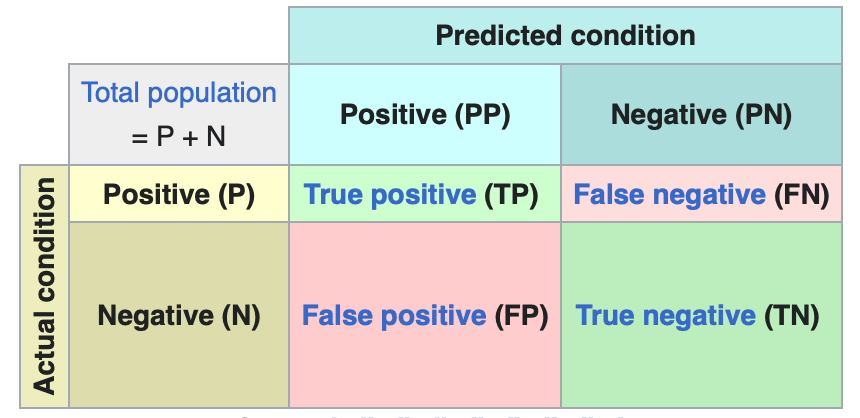
\includegraphics[width=0.75\linewidth]{assets/confusion_matrix.png}
  	\captionof{figure}{Confusion Matrix}
  	\label{fig:confusion_matrix}
\end{figure}

It summarises performance with the number of true positves (TP), true negatives (TN), false positives (FP) and false negatives (FN). 
What is a positive depends on the target class. In our case this is the class $1$ (the minority class) while a negative corresponds to class $0$ (the majority class).

From these values many standard measures are derived:

\textbf{Accuracy:}
Accuracy is the ratio between all that has been labeled correctly and the total number of samples, i.e.
\[
	\text{acc} = \frac{TP + TN}{TP + TN + FP + FN}
\]
It is a commonly used but fairly basic measure that often fails to accurately represent a classifiers performance in an imbalanced situation,
as for a high class imbalance the accuracy is high for a classifier that stubbornly predicts majority class for every sample.

\textbf{Sensitivity / True Positive Rate / Recall:}
Recall reflects the fraction of positive samples the classifier has identified i.e.
\[
	\text{rec} = \frac{TP}{TP + FN}
\]
It is more relevant in the imbalanced case as a classifier that chooses to label all before it as majority class to obtain good accuracy will have low recall.

\textbf{Precision:}
Precision represents the fraction of samples that have been correctly labeled positive i.e.
\[
	\text{prec} = \frac{TP}{TP + FP}
\]
This measure allows to assess whether the classifier tends to be correct when labelling a sample as minority class.

\textbf{Specificity:}
Gives the fraction of samples classified as correctly negative versus all negatives.
\[
	\text{spec} = \frac{TN}{TN + FP}
\]
Specificity is especially important when assessing the frequency and potential cost of false positives.

We have already described four different measures based on the confusion matrix, each of them assessing different aspects of the performance of a classifier.
But since all of these contribute important information, and since a classifier can have good scores in one but bad scores in another, 
how can one give a unified answer to the question "How good is my classifier?" when it comes to evaluation and decision making?
This question is the idea for the measures that follow.

One measure that intends to combine at least two of the metrics mentioned above is the \textbf{F1-score}.
It is the harmonic mean of precision and recall, where the harmonic mean for a set of positive real numbers $x_1, \dots, x_n$ is given by
\[
	H(x_1, \dotsm x_n) = \frac{n}{\sum_{j=1}^n \frac{1}{x_j}}
\]
which applied to precision and recall becomes
\[
	F = \frac{2}{ \frac{1}{\text{rec}} + \frac{1}{\text{prec}} } = 2 \frac{\text{rec} \, \text{prec}}{ \text{rec} + \text{prec} }.
\]
There are also weighted versions of the F1-score that are supposed to take into account whether recall or precision are more important in a given situation.

Given the test set the classifiers we used in our project predict the probabilities of class membership for each sample.
The standard way in which they then map these probabilities to a class prediction is by simply predicting the class with the largest probability.

Another important measure that provides a more comprehensive assessment of a classifiers performance is the \textbf{Receiver Operator Characteristic (ROC)}.
On a theoretical level, supposing here $X$ is the random variable representing the distribution of the feature vectors 
and our classifier outputs a continuous probability score $s(X)$, the ROC is obtained by considering different cutoff thresholds for that score.
Set the threshold $\tau$ to decide the predicted class such that if $s(X) > \tau$, we predict the positive class. 
Then the true positive rate (TPR) and the false positive rate (FPR) are given by
\[
    	\begin{aligned}
    		TPR(\tau) &= \mathbb{P}(s(X) > \tau | Y = 1) \\
    		FPR(\tau) &= \mathbb{P}(s(X) > \tau | Y = 0)
    	\end{aligned}
\]
where $Y$ is the r.v. representing the true class of $X$ for every realisation. 
TPR is the probability that the classifier ranks a randomly chosen positive instance higher than a randomly chosen negative instance. 
Similarly, FPR is the probability that the classifier ranks a randomly chosen negative instance higher than a randomly chosen positive instance.
    
The ROC curve plots $TPR(\tau)$ against $FPR(\tau)$ for all possible thresholds $\tau$, producing a curve that ranges from $(0,0)$ to $(1,1)$.
We can interpret a ROC plot as plotting the path of a function
\[
	f: \mathbb{R} \to [0,1]^2, \quad  \tau \mapsto (TPR(\tau), FPR(\tau))
\]
The \textbf{Area Under the ROC Curve (AUC)} then provides a single scalar value that represents the expected performance of the classifier.
An AUC of $1$ indicates a perfect classifier, while an AUC of $0.5$ indicates a classifier that performs no better than random chance.

AUC can also be interpreted in terms of the probability that the classifier will rank a randomly chosen positive instance higher than a randomly chosen negative instance,
assuming that one positive and one negative instance are chosen at random.

In practice ROC curves and AUC values are obtained by sorting the classified samples by score thus AUC is essentially a rank order statistic.


\subsubsection{Decision Theoretic Measures}
For example in a clinical setting this approach may be flawed however. 
Suppose the classifier is presented with mammography image data and the predicted probabilities for cancer in a case are $49\%$ for class $0$ (i.e. healthy tissue)
and $51\%$ for class $1$ (i.e. malignancy). The classifier would confidently predict a cancer diagnosis that may incur a risky biopsy for the patient.
Depending on the circumstances one might want to adapt or at least assess the probability threshold at which the classifier predicts class $1$.
To assess a classifiers performance in a context like this measures have been proposed that take into account the predicted probabilities and the risks involved.

\textbf{Risk Threshold}
Suppose r.v. $Y$ with outcome diseased $D$ or healthy $\neg D$.
Let $c_{TP}, c_{FP}, c_{TN}, c_{FN}$ then expected cost of predicting $\neg D$ is
\[
	\mathbb{P}(Y = 1) c_{FN} + \mathbb{P}(Y = 0) c_{TN}
\]

and expected cost for predicting $D$ is
\[
	\mathbb{P}(Y = 1) c_{TP} + \mathbb{P}(Y = 0) c_{FP}
\]

If we write $T = \mathbb{P}(Y = 1)$ we can rewrite to
\[
	T c_{FN} + (1-T) c_{TN}
\]
and
\[
	T c_{TP} + (1-T) c_{FP}
\]
One is indifferent about treatment if both expected costs are equal.
\[
\begin{aligned}
	T c_{FN} + (1-T) c_{TN} &= T c_{TP} + (1-T) c_{FP} \\
	&\Leftrightarrow \\
	T &= \frac{c_{TN} - c_{FP}}{(c_{TN} - c_{FP}) + (c_{TP} - c_{FN})} \\
\end{aligned}
\]
It can also be rearranged in a different way
\[
\begin{aligned}
	T c_{FN} + (1-T) c_{TN} &= T c_{TP} + (1-T) c_{FP} \\
	&\Leftrightarrow \\
	\frac{T}{1 - T} &= \frac{ c_{TN} - c_{FP} }{ c_{TP} - c_{FN} } \\
\end{aligned}
\]

In the first group, the costs relate to undertreatment (false-negative classifications)
The costs of these false-negative classifications $c_{FN}$ should be compared to the costs of true-positive classifications $c_{TP}$.
The difference $c_{TP} - c_{FN}$ is the net benefit of treating all who have the disease compared to treating none of them.
Suppose you have a treatment that causes lots of damage as well as curing the disease. 
Then this difference might be low, i.e. treating everyone with the dangerous treatment does not give much better outcome than simply not treating anyone.
Suppose on the other hand you have a devastating disease like Polio and a low cost treatment like a Polio-vaccine, then that difference will be strongly positive.

In the second group, relevant costs are for those without the event if not treated, who are treated (“overtreated”).
The costs of these false-positive classifications ($c_{FP}$) should be compared to the costs of true-negative classifications ($c_{TN}$)
while $c_{TN} - c_{FP}$ is the harm of treating all who don't have the disease compared to the benefit of not treating any of them.
E.g. the cost of not treating anyone without the disease might be 0 but the cost of treating them might be high. Then this value is strongly negative.
On the other hand suppose again a low impact vaccine that barely does harm, then that difference may be small negative. 

Odds (cutoff) = Harm/Benefit

The ratio in case of e.g. the polio vaccine could be strongly in favour of treating everyone (small cost for those without, high benefit for those with disease).


\textbf{Net Benefit}
The choice of risk threshold implicitly conveys the adopted relative misclassification costs. 
It can be derived that the odds of the risk threshold equal the harm-to-benefit ratio, which is the harm of a false positive divided by the benefit of a true positive.
For example, if a risk threshold of $20\%$ is used, the odds are 1 to 4. 
Therefore, a $20\%$ risk threshold assumes that the harm of a false positive is one-quarter of the benefit of a true positive or that 1 true positive is worth 4 false positives: 
A clinician might express this in terms such as ‘‘I would not do more than five biopsies to find one cancer.’’ 
Hence, when applying a model to a set of patients,
we can correct the number of true positives (TP) for the number of false positive (FP) using the odds $w$ of the risk threshold $t$: 
\[
	\text{TP} - w \text{FP} = \text{TP} - \frac{\tau}{1-\tau} \text{FP}
\]
When dividing by the total sample size $N$, the Net Benefit is obtained
\[
	\text{NB} = \frac{1}{N} (\text{TP} - w \text{FP}) = \frac{1}{N} (\text{TP} - \frac{\tau}{1-\tau} \text{FP})
\]

The Net Benefit of treat-none is always 0, 
whereas the Net Benefit of treat-all is positive for risk thresholds below the event rate and negative for risk thresholds above the event rate.
	
	
\subsection{Calibration}
Another key property of a prediction model is calibration, i.e., the agreement between observed outcomes and predictions.
\[
	TPR(\tau) = \mathbb{P}(s(X) > \tau | Y = 1)
\]


\subsection{Mixed}
	\begin{align*}
    		\color{teal} TPR(\tau) &= \mathbb{P}(s(X) > \tau | Y = 1) \\
    		\color{purple} FPR(\tau) &= \mathbb{P}(s(X) > \tau | Y = 0) \\
    	\end{align*}


\begin{comment}
\subsection{Accuracy rate}

	If benefit and harm are weighted equally, the odds of the threshold is 1:1, or a threshold probability of $50\%$. 
	This cutoff is by default considered in the calculation of the error rate, which is defined as (FN + FP)/N. 
	The complement is the accuracy rate: (TN + TP)/N.
	Often FN classifications are more important than FP classifications, which makes the accuracy rate not a sensible indicator of clinical usefulness.
	Other disadvantages include that the accuracy rate by definition is high for a frequent or infrequent outcome (i.e. imbalanced data).
	
	The accuracy rate is usually calculated at the simplistic cutoff of $50\%$, but can also be calculated at clinically defendable thresholds. 
	The harm-to-benefit ratio that underpins the choice of the cutoff should then be used to calculate a weighted accuracy, or its complement, the weighted error rate.
	We can express the TN classifications in units of the TP classifications, such that the weighted accuracy is calculated as (TP + w TN)/n.
	
	The improvement that is obtained by making decisions based on predictions from the model is the difference between the weighted accuracy
	obtained with the model versus the weighted accuracy of the default policy.
\end{comment}
	

\section{Machine Learning Pipeline}

This project was focused on two aspects.
The first was creating a machine learning pipeline that could facilitate an easy way to conduct experiments on imbalanced data.
The second was to use it to conduct some experiments to show it functions and to gain some additional insight into the imbalance problem itself.

Along the way we created three approaches to the pipeline, 
where the idea with each successive approach was to either improve generality and the potential scope of experiments that could be run,
or improve the efficiency of the pipeline computation- or memory-wise to obtain results quicker.
The fundamental layout of all three approaches was the same in the sense that each consisted of four or five python classes:
\begin{enumerate}[label=\arabic*)]
\item A \textbf{generator} class that creates the input data for a variety of parameters like the number, dimensionality and imbalance ratio of the samples
\item A \textbf{balancer} class that subjects the created data to a chosen balancing method to remedy the class imbalance
\item A \textbf{classifier} class that trains a chosen classifier on the output of the balancer class and conducts predictions on the test-set
\item An \textbf{metrics} or \textbf{assessor} class that applies standard metrics of classification quality to the predictions or guides the flow of the pipeline
\end{enumerate}

The first version of the pipeline is essentially a more elegant packaging for the application of methods from \texttt{scikit-learn}, \texttt{imblearn}, 
and some more specialised libraries like \texttt{xgboost}. 
In this version both the balancer and classifier classes are essentially just wrappers that invoke the balancing, 
training and prediction methods of the imported classes from these libraries.
Experiments are conducted directly via for-loop iteration over the experiment parameters.

The second approach was based on two ideas. One is to incorporate a new generator that allows more flexible generation of feature data.
The \texttt{make\_classification} method used in the first approach creates clusters exclusively with Gaussian features and does not allow to specify means or variances.
We created an own generator to amplify the control over and the variety of our sample distributions.
The other idea was to expand the functionality of the balancer and classifier classes by locating parts of the necessary iterations in a larger experiment in these classes.
The hope was to allow brief experiments to be conducted in a more modularised way and improve efficiency.
Since the goal of better efficiency was not achieved in this case we created a third approach.

Our third approach was mainly focused on computational efficiency. 
Stacked for-loop iterations turned out to be fairly slow and required a large amount of time to complete.
This is to some extend inevitable as the involved algorithms are complex and the datasets large, 
but the previous pipelines also created large additional overhead this approach was intended to reduce.

In the following we give a more detailed description of the created pipeline versions.

\subsection{First pipeline approach}

%.....


\subsection{Generator Generalisation and Localised Iteration Approach}

%......


\subsection{Fast Pipeline Approach}

Conducting an experiment with the two previous versions of the pipeline involves concatenated for-loop iterations over the respective parameter sets.
At each step of an iteration the data is passed between the active class instances of the pipeline and subsequently stored as an instance attribute before transformation.
There are two main sources of overhead that these approaches incur due to these operations.
For one, every iteration involves the creation and subsequent destruction of large arrays in memory, 
and while \texttt{numpy}'s C implementation guarantees efficient calculations on arrays of fixed size, 
creation of these arrays incurs significant overhead as large contiguous blocks of memory have to be reserved and released.
Secondly, at each step of an iteration the data is passed, i.e. copied, 
between the individual pipeline components, which again incurs the overhead due to creation and garbage collection.

The key idea of the last pipeline approach is to reduce the impact of these sources of overhead by creating large numpy arrays of adequate dimensions once,
giving each component of the pipeline a reference to the data instead of a copy, and applying the algorithms directly to sections of these large arrays.

To this end we introduce an intermediate parent class which only has an empty dictionary as a class attribute:
\begin{lstlisting}[language=Python, numbers=none]
class Data():

    	data_dict = {}
\end{lstlisting}

The other classes inherit from \texttt{Data} and modify the contents of the \texttt{data\_dict} dictionary.
To direct this process and create the necessary \texttt{numpy} arrays we created the \texttt{Assessor} class.
The \texttt{Assessor} takes in the \texttt{test\_size}, a list of dictionaries for the generator, and as before, a dictionary each for the balancers and classifiers to be used.
Its \texttt{\_\_init\_\_} method looks like this

\begin{lstlisting}[language=Python, numbers=none]
class Assessor(Data):

    def __init__(self, test_size, generation_dict_list, balancers_dict, classifiers_dict):

        Data.data_dict = {}

        self.test_size = test_size
        self.generation_dict_list = generation_dict_list

        balancer_list = [(name, balancer) for name, balancer in balancers_dict.items()]
        
        clsf_list = [(name, classifier) for name, classifier in classifiers_dict.items()]

        self.exp_dim = (len(generation_dict_list), len(balancers_dict), len(classifiers_dict))
        
        self.data_dict['assignment_dict'] = {(a, b, c): [gen_dict, bal, clsf]
                                             for (a, gen_dict), (b, bal), (c, clsf)
                                             in product(enumerate(generation_dict_list), 
                                                        enumerate(balancer_list), 
                                                        enumerate(clsf_list)
                                                        )
                                            }

\end{lstlisting}

Here the baseline dimensions for the \texttt{numpy} arrays that are to be created are calculated and saved in \texttt{self.exp\_dim} and 
the generation dictionaries and the names and classes corresponding to the balancers and classifiers are stored in the \texttt{assignment\_dict} 
under a three dimensional tuple key. 
This dictionary is essential to assign the methods to the correct positions in the later steps and the correct labels in the output files.

After initialisation the following methods are to be called in sequence if one wishes to execute the pipeline. 
In the generation function below we first check for the largest number of samples and dimensions to accommodate, 
then four \texttt{numpy} arrays of that size are created and filled with\texttt{np.nan} values.
Subsequently we iterate over the generation dictionaries in the stored list and assign a generation index to place the generated data in the correct part of the raw data arrays.
For each generation dictionary the \texttt{FMPL\_Generator} class is instantiated and its \texttt{prepare\_data} method is executed.
\begin{lstlisting}[language=Python, numbers=none]
def generate(self):     

	test_size = self.test_size
	table_infos = [extract_table_info(generation_dict) for generation_dict in self.generation_dict_list]
	
	self.d = max([info[0] for info in table_infos])
	n = max([info[1] for info in table_infos])
	a = self.exp_dim[0]
	        
	trainset_size = int((1-test_size)*n)
	testset_size = int(test_size*n)
	
	self.data_dict['org_X_train'] = np.full(shape = (a, trainset_size, self.d), fill_value = np.nan)
	self.data_dict['org_y_train'] = np.full(shape = (a, trainset_size,), fill_value = np.nan)
	
	self.data_dict['org_X_test'] = np.full(shape = (a, testset_size, self.d), fill_value = np.nan)
	self.data_dict['org_y_test'] = np.full(shape = (a, testset_size,), fill_value = np.nan)
	
	for i, generation_dict in enumerate(self.generation_dict_list):
		generation_dict['gen_index'] = i
		generator = FMPL_Generator(**generation_dict)
		generator.prepare_data(self.test_size)
\end{lstlisting}

The \texttt{FMPL\_Generator} doesn't differ much from the generator in the previous section apart from inheriting from \texttt{Data} and the \texttt{prepare\_data} method,
which now doesn't return the split raw data but instead inscribes it in the data arrays instantiated earlier.

The next method in line is the \texttt{balance} method. It is called with \texttt{bal\_params\_dicts} as a parameter that defaults to an empty dictionary.
This parameter is supposed to be a dictionary of dictionaries where each key should be a balancers name and the corresponding value should be a dictionary 
that contains the instantiation parameters of the balancer, most importantly the \texttt{'sampling_strategy'}.

\begin{lstlisting}[language=Python, numbers=none]
    def balance(self, bal_params_dicts = {}):

        a, b, c = self.exp_dim
        y_train = self.data_dict['org_y_train']

        default_strategy = 'auto'
        max_c1 = max([np.sum(y_train[data_ind] == 1) for data_ind in range(a)])
        max_total_samples = 0

        for data_ind in range(a):
            #check if a balancer parameter dict is given
            if bal_params_dicts:
                #iterate over the parameter dictionaries that are given
                for bal_dict in bal_params_dicts.values():

                    max_total_samples = max(max_total_samples, sum(calculate_no_samples(y_train[data_ind], bal_dict['sampling_strategy']).values()))

            #compare to default strategy if not every balancer has a dict
            if len(bal_params_dicts) < b:
                max_total_samples = max(max_total_samples, sum(calculate_no_samples(y_train[data_ind], default_strategy).values()))
        
        k = max_c1 + max_total_samples

        self.data_dict['bal_X_train'] = np.full(shape = (a, b, k, self.d), fill_value = np.nan)
        self.data_dict['bal_y_train'] = np.full(shape = (a, b, k, ), fill_value = np.nan)

        data_balancer = FMPL_DataBalancer(bal_params_dicts)
        
        data_balancer.balance_data()
\end{lstlisting}

The most complicated part of this step was to find the maximal number of samples for which to reserve space in the balanced data arrays.
\texttt{Imblearn} balancers allow a wide range of options to set the \texttt{'sampling_strategy'} and depending on which strategy the user settles on,
the final amount of samples varies drastically. This approach to the pipeline in general sacrifices memory consumption for faster execution time, 
but optimally the created arrays should not be much larger than they have to be to accommodate the data. 
To achieve an array that is as small as possible but as large as necessary the \texttt{calculate_no_samples} function calculates the number of samples
that can be expected depending on the sampling strategy and uses the maximum number among all balancers and datasets to be balanced.

\begin{lstlisting}[language=Python, numbers=none]
    def clsf_pred(self):

        a, n = np.shape(self.data_dict['org_y_test'])

        self.data_dict['clsf_predictions_y'] = np.full(shape = self.exp_dim + (n,), fill_value = np.nan)
        self.data_dict['clsf_predictions_proba'] = np.full(shape = self.exp_dim + (n, 2), fill_value = np.nan)
        self.data_dict['classes_order'] = np.full(shape = self.exp_dim + (2,), fill_value = np.nan)

        print('Size classifier array: \n', self.exp_dim[0]*self.exp_dim[1]*self.exp_dim[2]*n*2)
        data_classifier = FMPL_DataClassifier()

        data_classifier.fit()

        data_classifier.predict()

\end{lstlisting}

\begin{lstlisting}[language=Python, numbers=none]

    def calc_metrics(self, std_metrics_dict = {}):

        default_metrics = {
            'accuracy': accuracy_score,
            'precision': precision_score,
            'recall': recall_score,
            'F1 score': f1_score,
            'ROC AUC Score': roc_auc_score,
        }

        metrics_dict = std_metrics_dict or default_metrics


        self.data_dict['std_metrics_res'] = np.full(shape = self.exp_dim + (len(metrics_dict),), fill_value = np.nan)
        
        metrics = FMPL_Metrics(metrics_dict)

        metrics.confusion_metrics()

        std_metrics_res = self.data_dict['std_metrics_res'].reshape(-1, len(metrics_dict))

        results_df = pd.DataFrame(std_metrics_res, columns= [name for (name, metr_func) in metrics.std_metric_list])

        reference_list = [self.data_dict['assignment_dict'][(i, j, k)] 
                          for i in range(self.exp_dim[0]) 
                          for j in range(self.exp_dim[1]) 
                          for k in range(self.exp_dim[2])]

        reference_list = [extract_table_info(alist[0])+[alist[1][0], alist[2][0]] for alist in reference_list]

        reference_df = pd.DataFrame(reference_list, columns= ['n_features', 
                                                              'n_samples', 
                                                              'class_ratio', 
                                                              'distributions', 
                                                              'balancer', 
                                                              'classifier'])

        results_df = pd.concat([reference_df, results_df], axis = 1)

        return results_df
\end{lstlisting}


%\subsection{Pipeline description}



\section{Experiments and Results}

There are an abundance of papers and studies that investigate the effect of imbalanced data and the diverse balancing algorithms in classification.
While researching for this project we saw many evaluation tables representing the performance of binary classifiers in a variety of circumstances.
We concluded that obtaining comprehensive results is beyond the scope of this team project, but we conducted experiments 
and we hope they can add something of value to the existing research, or at the very least, give the reader an overview of the overall challenges and tradeoffs involved.

There are some common truths established in previous research that we can state in advance.
For one, the number of available samples and the class imbalance ratio have a great effect on the success of any balancing method and classifier.
If there are only a handful of samples of the minority class available, because either the sample size is too low or the imbalance ratio to steep,
then no balancer or classifier will perform well.
One can also not hope for good performance if the number of features in which the class distributions have significant differences is too low, or
the sample clusters have too much overlap.

Our first experiment investigates this effect of class cluster distance in a simplified context of standard multivariate normal distributions.


\subsection{Cluster Distance Experiment}

When we conducted this experiment with the custom generator described in the previous section we came up with a function 
that generated the necessary parameter dictionaries for a standard multivariate distribution of i.i.d. components.
The idea was to have the mean of one cluster situated at the origin and the mean of the other at varying distance from it in the first orthant with all feature component
values being equal. We derived the corresponding for the latter mean like this:

Given a euclidian distance $d$ from the origin in $\mathbb{R}^n$, the coordinates of a vector $x \in \mathbb{R}^n$ with $x_1 = \dots = x_n$ are given by
\[
\begin{aligned}
	& \, d = \sqrt{ \sum_{j =1}^n x_j^2} = \sqrt{ n x_j^2} \\
	\Leftrightarrow& d^2 = n x_j^2 \\ 
	\Leftrightarrow& x_j = \frac{d}{\sqrt{n}} \\ 
\end{aligned}
\]

This formula for the coordinate components shows one of the faces of the phenomenon known as the "curse of dimensionality".
As the number of dimensions, $n$ in this case, increases the magnitude of the individual feature components decreases, bringing them closer to the origin.
So while the euclidian distances may be the same, the individual components of each cluster move closer together.
An algorithm that attempts to distinguish the clusters component-wise (as is necessary in the independent case we assume) will hence struggle severely to
distinguish the classes in higher dimensions. This is also what we observed in practice.

We ran the experiment with the FMLP pipeline using all combinations of unbalanced data, data balanced by \texttt{SMOTE}, \texttt{ADASYN}, \texttt{BorderlineSMOTE} and 
\texttt{SVMSMOTE} and the classifiers \texttt{LogisticRegression}, \texttt{DecisionTreeClassifier}, \texttt{Random Forest}, \texttt{XGboost} and \texttt{Lightgbm}.
These were used for all combinations of data with $10.000$ and $100.000$ samples, class ratios of $10\%$, $1\%$ and for $100.000$ also $0.1\%$ minority class,
and feature numbers $2,4,6,8$.
This produced a large table of some $4000$ entries that we intend to summarise here.

\begin{comment}
% for some reason this block does not work at all, while the others do
%\begin{tabular}{|r*{6}{|c}|}
\begin{tabular}{|*{6}{|c}|}
	\bfseries {cluster distance} & \bfseries accuracy & \bfseries precision & \bfseries  recall & \bfseries {F1 score} & \bfseries {ROC AUC Score} \\% specify table head
	%cluster distance & accuracy & precision & recall & F1 score &  ROC AUC Score % specify table head
	\csvreader[head to column names]{assets/tables/distance_mean_values.csv}{}{
	\csvcoli & \csvcolii & \csvcoliii & \csvcoliv & \csvcolv  & \csvcolvi %\thecsvrow &
	}% specify your coloumns here
	\\\hline
\end{tabular}
\end{comment}

We obtained the following table by grouping by the cluster distance and taking the mean across entries.
\begin{table}[H]
\centering
%\csvautotabular{assets/tables/distance_mean_values.csv}
\csvreader[
	tabular = *{6}{|c}|,
	table head = \hline \bfseries {cluster distance} & \bfseries accuracy & \bfseries precision & \bfseries  recall & \bfseries {F1-score} & \bfseries {ROC AUC Score}\\\hline, 
	late after line = \\\hline
	]{assets/tables/distance_mean_values.csv}{}{%
	\csvcoli & \csvcolii & \csvcoliii & \csvcoliv & \csvcolv  & \csvcolvi
}
\caption{Table aggregated by cluster distance}
\end{table}

What comes as no surprise is that the performance in every standard metric is on average better, the further the clusters are apart. 
Interestingly accuracy remains relatively high even for low distances while precision and F1-score decline dramatically when the clusters are close.
This demonstrates the "inadequacy of accuracy" (cite) as a measure of classifier performance in this context.

For sample sizes of $100.000$ and class ratio $0.1\%$ the balancing process failed at cluster distance $1$. 
At this point the clusters have some much overlap and the minority class is in comparison so underrepresented 
that attempting to find a minority class nearest neighbour to a minority class sample is often in vain.
Another interesting insight is that in general the balancing step takes significantly longer the lower the distance between the clusters.
At a distance of $4$ or $5$ FMLP completes the balancing step in seconds, while at a distance of $1.5$ or $1$ this step took up to half an hour to complete or failed entirely.

When we instead group and aggregate the performance metrics by the balancer used we obtain the following table:

\begin{table}[H]
\centering
%\csvautotabular{assets/tables/distance_mean_values.csv}
\csvreader[
	tabular = *{6}{|c}|,
	table head = \hline \bfseries {balancer} & \bfseries accuracy & \bfseries precision & \bfseries  recall & \bfseries {F1-score} & \bfseries {ROC AUC Score}\\\hline, 
	late after line = \\\hline
	]{assets/tables/dist_bal_mean_values.csv}{}{%
	\csvcoli & \csvcolii & \csvcoliii & \csvcoliv & \csvcolv  & \csvcolvi
}
\caption{Table aggregated by balancing method}
\end{table}

We can see that both recall and AUC values are on average significantly improved by balancing the data.
Precision however can be seen to decrease across balancing algorithms compared to training on unbalanced data.
Considering that recall is higher but precision is lower we can conclude that the overall rate of false positives increases when using a balancing algorithm.
This is most likely due to the often criticised (cite) tendency of balancing methods to lead to systematic over-prediction of minority class probabilities.
We will show this tendency more clearly in the section on calibration curves.

For completeness we also aggregated by classification method.

\begin{table}[H]
\centering
%\csvautotabular{assets/tables/distance_mean_values.csv}
\csvreader[
	tabular = *{6}{|c}|,
	table head = \hline \bfseries {classifier} & \bfseries accuracy & \bfseries precision & \bfseries  recall & \bfseries {F1-score} & \bfseries {ROC AUC Score}\\\hline, 
	late after line = \\\hline
	]{assets/tables/dist_clsf_mean_values.csv}{}{%
	\csvcoli & \csvcolii & \csvcoliii & \csvcoliv & \csvcolv  & \csvcolvi
}
\caption{Table aggregated by classification method}
\end{table}

The scores are fairly similar, but what seemed surprising to us was that a simple decision tree, which we mainly included for reference, 
performed only marginally worse than its corresponding ensemble method: random forest.


\subsection{Mode Experiment}

For this experiment we attempted to investigate how a situation, where one of the class distributions is bimodal, affects the outcome of the balancing and classification steps.
We set the clusters
The first case we are going to look at is that the majority class  

















\subsection{Hypothesis testing}
The \textbf{Hypothesis-T-Test} class is designed to facilitate hypothesis testing, specifically t-tests, on datasets stored in CSV format. It enables us to compare the effectiveness of different combinations of data balancing and classification methods in terms of key performance measures. The t-test is an appropriate choice in this case, where we want to apply multiple pairwise comparisons of continuous variables (the target measures). Hereby is an overview of its functionality.

The class constructor accepts several essential parameters: 
\begin{enumerate}[label=$\bullet$]
\item \textbf{target list}: a list of target performance measures;
\item \textbf{column bal}: the name of the file column addressing the data balancing method
\item \textbf{column clas}: the name of the file column addressing the classifier method
\item \textbf{test combination balancers}: a list of tuples, each containing a combination of two balancing methods for comparison
\item \textbf{test combination classifiers}: a list of tuples, each containing a combination of two classifier methods for comparison
\item \textbf{alpha}: the test significance level, set by default to 0.05, a typical choice in hypothesis testing. 
\end{enumerate}

The core functionality of the class resides in the \textbf{perform-t-test} method, which consists of the following steps:
\begin{enumerate}[label=$\bullet$]
\item Initialization of an empty list, \textbf{results}, to store the outcomes of the t-tests.
\item For each target performance measure, the class iterates through the provided combinations of balancing methods and classifier methods.
\item The data is filtered based on the selected balancing or classifier method, creating two distinct groups.
\item A t-test is conducted on the two groups, producing statistical values such as the t-statistic and p-value.
\item The mean values of the target performance measure are calculated for each group.
\item The test results, including the target performance measure, compared methods, mean values, t-statistic, and p-value, are organized into dictionaries and appended to the \textbf{results} list.
\item After completing all t-tests, the results are compiled into a pandas DataFrame and saved to a CSV file. This file serves as a comprehensive record of the statistical comparisons.
\end{enumerate}

\subsection{Linear regression Analysis}
Another crucial step in our pipeline is to thoroughly explore the relationships between our target measures and the parameters of interest that we allowed to vary in the preceding stages of our project. To achieve this, we've developed the \textbf{Linear Regression Analysis} class. This class empowers us to conduct in-depth investigations into how specific predictor variables influence our chosen target metrics. In the following, we will delve into the functionality of this class and showcase its applications in our data analysis process.
After loading a dataset from a specified CSV file and storing it in a pandas DataFrame, the data need to be set up for regression analysis. This is done through the \textbf{prepare data} method, which takes two sets of input variables: categorical and continuous regressors. The categorical variables are encoded into binary format and combined with the continuous regressors to create the input matrix \textbf{X}.
The actual analysis is then implemented in the function \textbf{perform linear regression}, which takes the following inputs: 
\begin{enumerate}[label=$\bullet$]
\item \textbf{target}: the target metric that we want to predict
\item \textbf{regressors}: a list of predictor variables used in the regression analysis 
\end{enumerate}
The function performs the following steps: 
\begin{enumerate}[label=$\bullet$]
\item Splits the dataset into training and testing sets.
\item Fits a linear regression model to the training data.
\item Predicts the target metric for the test data.
\item Calculates various regression metrics, including mean squared error, mean absolute error, coefficient values, coefficient of determination (R-squared), F-value, and p-value.
\item Stores the results in a pandas DataFrame and returns it.
\end{enumerate}

Finally, the method \textbf{plot target vs regressors} repeats the analysis and loops through each regressor in the regressors list. For each regressor, the corresponding predicted values \textbf{y values} are calculated as a sum of the intercept and the product between the regression coefficients and the data. Next, a scatter plot is produced to graphically observe the relationship.



\begin{comment}
\begin{thebibliography}{9}

\bibitem{SMOTE}
 Nitesh, V., Chawla., Kevin, W., Bowyer., Lawrence, O., Hall., W., Philip, Kegelmeyer. (2002). SMOTE: synthetic minority over-sampling technique. Journal of Artificial Intelligence Research, 16(1):321-357. doi: 10.1613/JAIR.953


\bibitem{ADASYN}
 Haibo He, Yang Bai, E. A. Garcia and Shutao Li, "ADASYN: Adaptive synthetic sampling approach for imbalanced learning," 2008 IEEE International Joint Conference on Neural Networks (IEEE World Congress on Computational Intelligence), Hong Kong, 2008, pp. 1322-1328, doi: 10.1109/IJCNN.2008.4633969.
 
\end{thebibliography}	
\end{comment}

\section{References}
\bibliographystyle{plain} % We choose the "plain" reference style
\bibliography{assets/references} % Entries are in the refs.bib file




\end{document}
